\documentclass[11pt,letter]{article}
\usepackage{amsmath}
\usepackage{amssymb}	% packages that allow mathematical formatting
\usepackage{graphicx}	% package that allows you to include graphics
\usepackage{setspace}	% package that allows you to change spacing
\usepackage{fullpage}	% package that specifies normal margins
\usepackage{microtype}
\usepackage{amsthm}
\newcommand{\argmin}{\operatornamewithlimits{argmin}}
\renewcommand\qedsymbol{$\blacksquare$}
\usepackage{listings}
\usepackage{color}
\usepackage{subfig}


\definecolor{codegreen}{rgb}{0,0.6,0}
\definecolor{codegray}{rgb}{0.5,0.5,0.5}
\definecolor{codepurple}{rgb}{0.58,0,0.82}
\definecolor{backcolour}{rgb}{0.95,0.95,0.95}

\lstdefinestyle{mystyle}{
	backgroundcolor=\color{backcolour},   
	commentstyle=\color{codegreen},
	keywordstyle=\color{magenta},
	numberstyle=\tiny\color{codegray},
	stringstyle=\color{codepurple},
	basicstyle=\footnotesize,
	breakatwhitespace=false,         
	breaklines=true,                 
	captionpos=b,                    
	keepspaces=true,                 
	numbers=left,                    
	numbersep=5pt,                  
	showspaces=false,                
	showstringspaces=false,
	showtabs=false,                  
	tabsize=2
}

\lstset{style=mystyle}

%\usepackage[left=2.5cm, right=2.5cm, top=2cm, bottom = 3cm]{geometry}


	

\begin{document}

\begin{figure}
	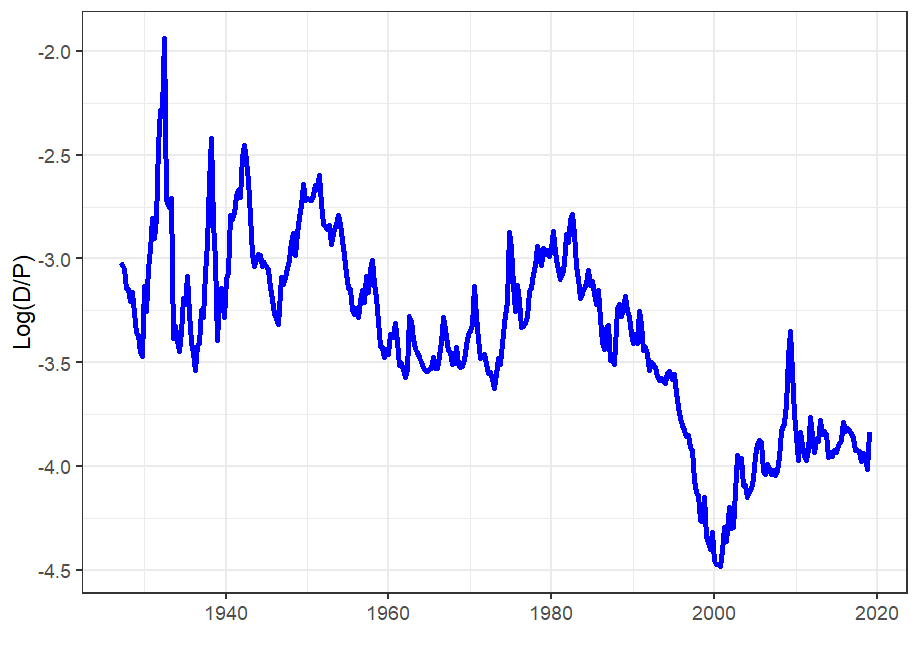
\includegraphics[width=\linewidth]{log_dividend_yield.png}
	\caption{Dividend yield (sum of past years worth of dividends divided by current portfolio price)}
	\label{fig:div_yield}
\end{figure}
We run two regressions separately of the form
\begin{equation*}
	\begin{split}
	r_{t, t+\tau} & = \alpha_r + \beta_{r, \tau}(d_t - p_t) + \epsilon^r_{t+\tau}\\
	\Delta d_{t, t+\tau} & = \alpha_{\Delta_d}+\beta_{\Delta d, \tau}(d_t - p_t)+ \epsilon^dp_{t+\tau}\\
	\end{split}
\end{equation*}
the results of which are shown in the tables below


\begin{table}[!htbp] \centering 
	\label{} 
	\begin{tabular}{@{\extracolsep{5pt}} cccc} 
		\\[-1.8ex]\hline 
		\hline \\[-1.8ex] 
		 $\tau$ & b & t(b) & r2 \\ 
		\hline \\[-1.8ex] 
		4 & $0.076$ & $2.541$ & $0.026$ \\ 
		12 & $0.209$ & $5.938$ & $0.073$ \\ 
		20 & $0.336$ & $9.144$ & $0.129$ \\  
		\hline \\[-1.8ex] 

	\end{tabular} 
	\quad
	\begin{tabular}{@{\extracolsep{5pt}} cccc} 
		\\[-1.8ex]\hline 
		\hline \\[-1.8ex] 
		$\tau$ & b & t(b) & r2 \\ 
		\hline \\[-1.8ex] 
		4 & -$0.093$ &-$6.614$ & $0.165$ \\ 
		12 & -$0.229$ & -$6.956$ & $0.197$ \\ 
		20 & -$0.364$ & -$8.757$ & $0.250$ \\  
		\hline \\[-1.8ex] 
	\end{tabular} 
			\caption{Return Regressions (left panel) and dividend growth regressions (right panel)} 
\end{table} 
We can infer how much of the variation in the price dividend ratio is due to variation in cash flows and how much is due to variation in future returns through the following decomposition. First, we can use the discount rate regression to calculate
\begin{equation*}
	r_{t+1} - E_t r_{t+1} = \epsilon_{t+1}
\end{equation*}
Then calculate discount rate news as
\begin{equation*}
	N_{DR, t+1} = \sum_{j=0}^{\infty} \kappa^j\beta_{r, j}^j\epsilon_{t+1}
\end{equation*}
since this regression implies $E_t r_{t+\tau} = \alpha + \beta^\tau(d_t-p_t)$. The cash flow news would then be
\begin{equation*}
	N_{CF, t+1} = r_{t+1} - E_t r_{t+1} + N_{DR, t+1}
\end{equation*}

\begin{table}[!htbp] \centering 
	\caption{} 
	\label{} 
	\begin{tabular}{@{\extracolsep{5pt}}lc} 
		\\[-1.8ex]\hline 
		\hline \\[-1.8ex] 
		& \multicolumn{1}{c}{\textit{Dependent variable:}} \\ 
		\cline{2-2} 
		\\[-1.8ex] &   \\ 
		\hline \\[-1.8ex] 
		dp:(Intercept) & $-$0.204$^{**}$ \\ 
		& (0.084) \\ 
		& \\ 
		dp:dp.l1 & 0.931$^{***}$ \\ 
		& (0.026) \\ 
		& \\ 
		dp:dgr.l1 & 0.157$^{*}$ \\ 
		& (0.081) \\ 
		& \\ 
		dp:rf.l1 & 0.990 \\ 
		& (0.763) \\ 
		& \\ 
		dp:trend & 0.000$^{***}$ \\ 
		& (0.000) \\ 
		& \\ 
		dgr:(Intercept) & $-$0.222$^{***}$ \\ 
		& (0.081) \\ 
		& \\ 
		dgr:dp.l1 & $-$0.079$^{***}$ \\ 
		& (0.027) \\ 
		& \\ 
		dgr:dgr.l1 & 0.575$^{***}$ \\ 
		& (0.090) \\ 
		& \\ 
		dgr:rf.l1 & 0.913 \\ 
		& (0.727) \\ 
		& \\ 
		dgr:trend & 0.000$^{*}$ \\ 
		& (0.000) \\ 
		& \\ 
		rf:(Intercept) & 0.000 \\ 
		& (0.001) \\ 
		& \\ 
		rf:dp.l1 & 0.000 \\ 
		& (0.000) \\ 
		& \\ 
		rf:dgr.l1 & 0.001$^{**}$ \\ 
		& (0.000) \\ 
		& \\ 
		rf:rf.l1 & 0.976$^{***}$ \\ 
		& (0.018) \\ 
		& \\ 
		rf:trend & 0.000 \\ 
		& (0.000) \\ 
		& \\ 
		\hline \\[-1.8ex] 
		\hline 
		\hline \\[-1.8ex] 
		\textit{Note:}  & \multicolumn{1}{r}{$^{*}$p$<$0.1; $^{**}$p$<$0.05; $^{***}$p$<$0.01} \\ 
	\end{tabular} 
\end{table}

\end{document}


